\documentclass{beamer}

% ===== 基础宏包 =====
\usepackage{ctex}
\usepackage{amsmath, amsfonts, amssymb, bm}
\usepackage{mathrsfs}
\usepackage{graphicx}
\usepackage{ragged2e}
\usepackage{hyperref}
\usepackage{booktabs}
\usepackage{array}

% ===== Beamer 主题设置 =====
\usetheme{Berlin}
\usecolortheme{whale}
\useinnertheme[shadow=true]{rounded}
\usefonttheme[onlymath]{serif}
\setbeamercovered{transparent}
\setbeamertemplate{navigation symbols}{}

% ===== 页脚设置 (修复了 hbox 溢出问题) =====
\setbeamertemplate{footline}{%
 \leavevmode%
 \hbox{%
 \begin{beamercolorbox}[wd=.31\paperwidth,ht=2.25ex,dp=1ex,center]{author in head/foot}
 \insertshortauthor
 \end{beamercolorbox}%
 \begin{beamercolorbox}[wd=.34\paperwidth,ht=2.25ex,dp=1ex,center]{title in head/foot}
 \insertshorttitle
 \end{beamercolorbox}%
 \begin{beamercolorbox}[wd=.31\paperwidth,ht=2.25ex,dp=1ex,center]{date in head/foot}
 \insertshortdate \quad \insertframenumber/\inserttotalframenumber
 \end{beamercolorbox}%
 }
}

% ===== 标题信息 =====
\title[Matbench 晶体性质预测学习汇报]{基于 Matbench 的晶体图神经网络性质预测学习汇报}
\author[刘嘉瑞]{汇报人：刘嘉瑞}
\institute[学习报告]{本周文献精读：ComFormer / MGT / HC-GNN / VGNN / Hamiltonian GNN / MACE}
\date{2026 年 4 月}

\begin{document}

% ===== 封面 =====
\begin{frame}
 \titlepage
\end{frame}

% ===== 目录 =====
\begin{frame}{目录}
 \tableofcontents
\end{frame}

\section{学习背景与问题主线}

\begin{frame}{学习背景：为什么继续往前看这 6 篇论文}
\begin{itemize}
  \item 目前已经成功复现 \textbf{CGCNN、ALIGNN、M3GNet}，对晶体图构建、键角建模、三体信息传播已有基础认识。
  \item 但现有基础模型仍有几个明显瓶颈：
  \begin{itemize}
    \item 晶体图表示对周期性与全局结构的编码仍不够充分；
    \item 长程相互作用、全局筛选机制较弱；
    \item 图结构大多仍是“平面原子图”，层级结构与虚拟节点用得较少；
    \item 强物理约束与高阶等变消息传递仍有较大提升空间。
  \end{itemize}
  \item 因此，本周围绕三个方向精读 6 篇文章，目标不是简单堆论文，而是为后续\textbf{改良晶体 GNN}打方法基础。
\end{itemize}
\end{frame}

\begin{frame}{本周精读的三条主线}
\begin{itemize}
  \item \textbf{方向一：图 Transformer 与长程注意力筛选机制}\\
        ComFormer、MGT：关注\textbf{周期性编码、全局信息交互、长程作用建模}。
  \vspace{1.5mm}
  \item \textbf{方向二：层级化 / 超节点 /虚拟节点架构}\\
        HC-GNN、VGNN：关注\textbf{多尺度图结构、超节点汇聚、变长输出}。
  \vspace{1.5mm}
  \item \textbf{方向三：强物理约束模型}\\
        Hamiltonian GNN、MACE：关注\textbf{更物理的输入表示、高阶等变消息传递}。
\end{itemize}

\vspace{2mm}
\hrule
\vspace{2mm}

\begin{itemize}
  \item 这三条主线分别对应：\textbf{表示升级、结构升级、物理约束升级}。
  \item 也是后续在现有基础（CGCNN/ALIGNN/M3GNet）上最值得推进的几个方向。
\end{itemize}
\end{frame}

\begin{frame}{六篇文章总览}
\small
\centering
\begin{tabular}{p{2.2cm} p{3.5cm} p{4.2cm}}
\toprule
论文 & 核心问题 & 对后续改良的启发 \\
\midrule
ComFormer & 完备晶体图表示、周期被动对称性 & 从晶体图表示层面升级 ALIGNN/M3GNet \\
MGT & 补足长程静电相互作用 & 构建 local/line/global 三图混合结构 \\
HC-GNN & 长程传播困难、缺乏层级结构 & 引入社区/基序超节点、多尺度消息传递 \\
VGNN & 谱类任务输出变长 & 用虚拟节点表示中间物理对象 \\
Hamiltonian GNN & 如何直接利用电子结构信息 & 以 Hamiltonian / orbital 为输入构图 \\
MACE & 高精度 many-body 等变建模 & 用高阶消息替代单纯堆深网络 \\
\bottomrule
\end{tabular}
\end{frame}

\section{方向一：图 Transformer 与长程注意力}

\begin{frame}{方向一：为什么要从局部消息传递走向全局筛选}
\begin{itemize}
  \item CGCNN 主要依赖局部邻域和距离；ALIGNN 补充了 line graph 与键角；M3GNet 进一步增强了几何建模。
  \item 但晶体任务中仍然存在两个难点：
  \begin{itemize}
    \item \textbf{几何表示是否完备}：能否区分不同周期晶体？
    \item \textbf{长程相互作用是否显式建模}：例如静电作用、跨局域单元的筛选机制。
  \end{itemize}
  \item 因此本方向主要看两篇：
  \begin{itemize}
    \item \textbf{ComFormer}：从晶体图表示与周期对称性切入；
    \item \textbf{MGT}：从 long-range interaction 与 attention 切入。
  \end{itemize}
\end{itemize}
\end{frame}

\begin{frame}[shrink]{ComFormer：完备晶体图表示 + Transformer}
\begin{columns}[T]
\column{0.64\textwidth}
\small
\begin{itemize}
  \vspace{-4mm}
  \item 正式标题：\textbf{Complete and Efficient Graph Transformers for Crystal Material Property Prediction}。
  \item 核心问题：现有晶体图往往不能同时处理\textbf{SE(3) 对称性 + periodic invariance}，因而表示不完备。
  \item 关键创新：
  \begin{itemize}
    \item 提出 invariant / equivariant crystal graph；
    \item 用每个原子的 lattice representation 编码周期信息；
    \item 设计 iComFormer 与 eComFormer 两个版本。
  \end{itemize}
  \item 我的理解：这篇论文最重要的价值在于回答了“\textbf{晶体图该怎样构，才配得上 Transformer}”。
\end{itemize}

\column{0.36\textwidth}
\centering
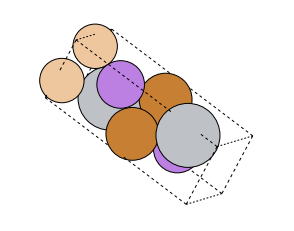
\includegraphics[width=0.85\linewidth]{figures/ComFormer_Complete_and_Efficient_Graph_Transformers_for_Crystal_Material_Property_Prediction_p4_1.png}\\
\vspace{1mm}
{\scriptsize 图：论文中关于晶体被动对称性/表示动机的示意}
\end{columns}
\end{frame}

\begin{frame}[shrink]{ComFormer 对现有研究基础的启发}
\begin{columns}[T]
\column{0.50\textwidth}
\small
\vspace{-3mm}
\textbf{接在现有基线之后怎么学：}
\begin{itemize}
  \item 对 CGCNN：补足仅靠距离难以表达晶体周期几何的缺陷；
  \item 对 ALIGNN：进一步追问“有角度还够不够”；
  \item 对 M3GNet：从势函数建模继续上探到\textbf{表示完备性}。
\end{itemize}

\textbf{后续可直接借鉴的点：}
\begin{itemize}
  \item 晶体图中显式编码晶胞周期向量；
  \item 将 invariant/equivariant 表示与 Transformer 结合；
  \item 在 Matbench 任务中验证全局建模是否稳定提升。
\end{itemize}

\column{0.50\textwidth}
\centering
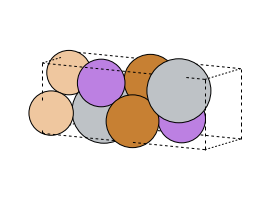
\includegraphics[width=0.85\linewidth]{figures/ComFormer_Complete_and_Efficient_Graph_Transformers_for_Crystal_Material_Property_Prediction_p6_1.png}\\
\vspace{1mm}
{\scriptsize 图：ComFormer 流程图/模块示意}
\end{columns}
\end{frame}

\begin{frame}[shrink]{Molecular Graph Transformer：从 ALIGNN 走向长程相互作用}
\begin{columns}[T]
\column{0.7\textwidth}
\small
\begin{itemize}
  \vspace{-4mm}
  \item 正式标题：\textbf{Molecular Graph Transformer: stepping beyond ALIGNN into long-range interactions}。
  \item 核心问题：局部图与线图对近邻化学环境刻画较强，但对\textbf{长程静电作用}仍不敏感。
  \item 关键创新：
  \begin{itemize}
    \item 构造 \textbf{local + line + global} 三图表示；
    \item 在 global graph 上使用 multi-head attention；
    \item 用类 Coulomb 特征显式建模长程静电作用。
  \end{itemize}
  \item 我的理解：这篇是最适合从 ALIGNN 自然延伸过去的文章——保留局部键角建模，同时补上全局筛选机制。
\end{itemize}

\column{0.36\textwidth}
\centering
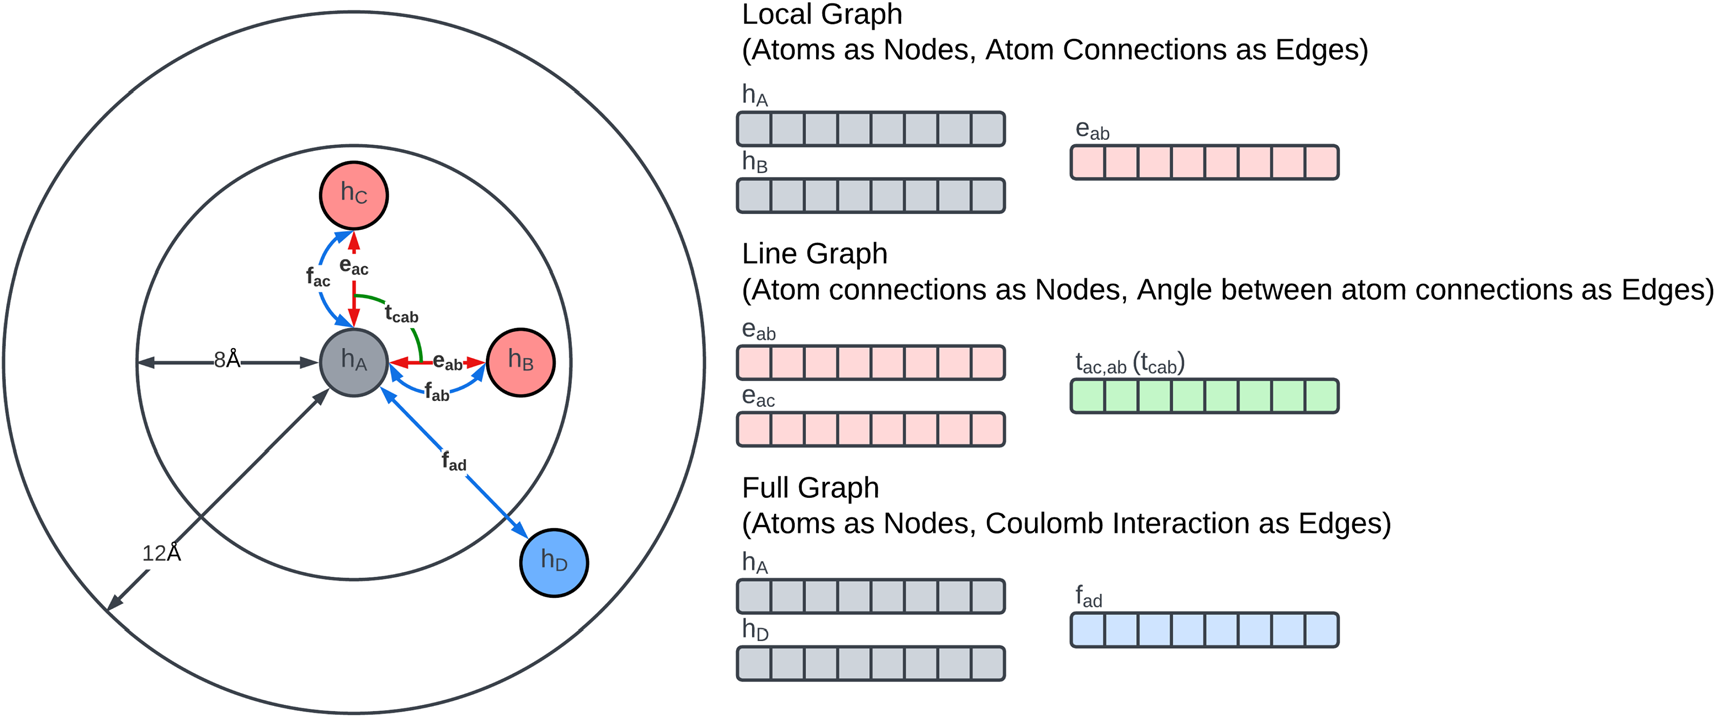
\includegraphics[width=0.85\linewidth]{figures/Molecular_Graph_Transformer_Stepping_Beyond_ALIGNN_Into_Long_Range_Interactions_p3_1.png}\\
\vspace{1mm}
{\scriptsize 图：MGR 三图表示（local/line/global）}
\end{columns}
\end{frame}

\begin{frame}[shrink]{方向一小结：ComFormer vs. MGT}
\begin{columns}[T]
\column{0.60\textwidth}
\small
\begin{itemize}
  \item \textbf{ComFormer} (几何表示论)：先把晶体图表示做对，再让 Transformer 发挥作用。
  \item \textbf{MGT} (任务驱动增强)：针对长程作用明确加 global graph 和 attention。
  \item \textbf{共同结论}：仅靠局部 message passing 已不够，后续模型必须更重视：
  \begin{itemize}
    \item 全局信息的显式筛选；
    \item 周期性与长程作用的结构化编码；
    \item 局部几何与全局作用的融合机制。
  \end{itemize}
  \item \textbf{直接启发}：可以尝试在现有框架里引入 \textbf{global graph / periodic encoding}。
\end{itemize}

\column{0.40\textwidth}
\centering
\vspace{4mm}
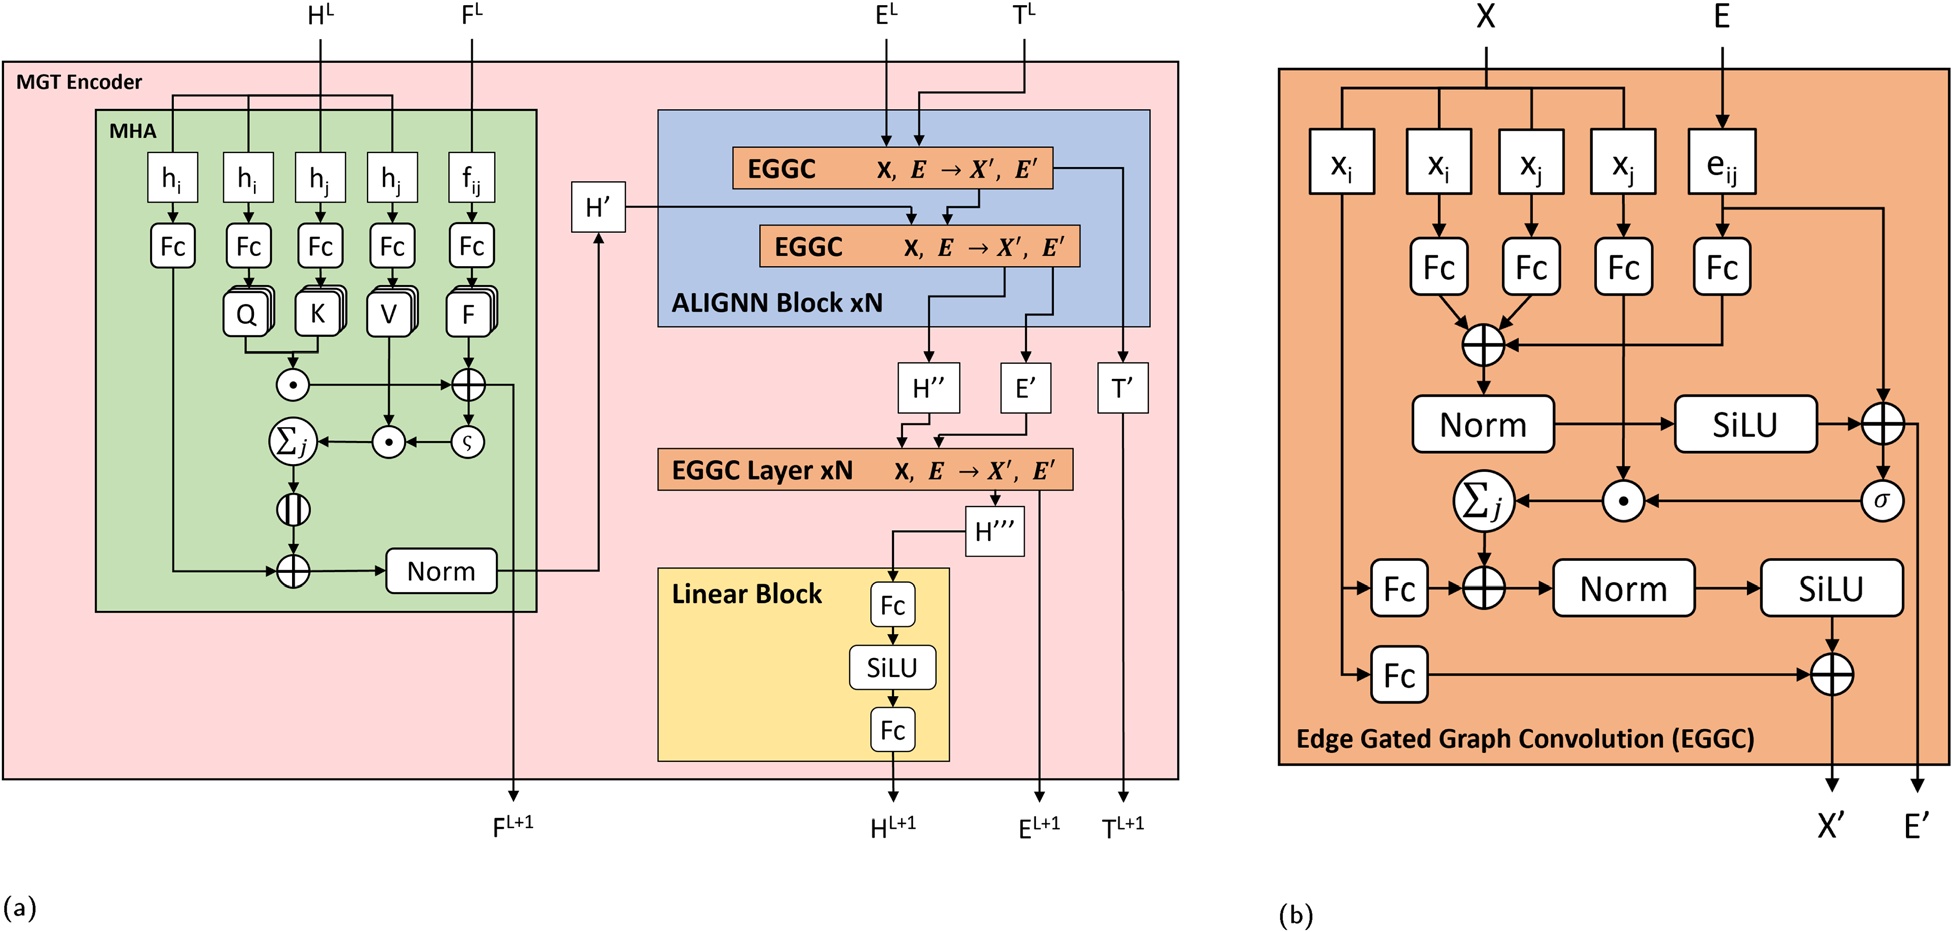
\includegraphics[width=0.85\linewidth]{figures/Molecular_Graph_Transformer_Stepping_Beyond_ALIGNN_Into_Long_Range_Interactions_p4_1.png}
\end{columns}
\end{frame}

\section{方向二：层级化与虚拟节点架构}

\begin{frame}{方向二：为什么要引入层级结构与虚拟节点}
\begin{itemize}
  \item 传统晶体 GNN 往往默认：\textbf{原子就是全部节点，图边就是全部关系}。
  \item 但很多任务并不适合只在平面原子图上做消息传递：
  \begin{itemize}
    \item 长程传播会出现 over-squashing；
    \item 晶体中的局部基序/多面体/团簇语义没有被显式表达；
    \item 谱类任务（如 phonon dispersion）输出维度随结构变化，普通 pooling 不够自然。
  \end{itemize}
  \item 因此本方向重点看：
  \begin{itemize}
    \item \textbf{HC-GNN}：图结构做层级化；
    \item \textbf{Virtual Node GNN}：节点功能做扩展化。
  \end{itemize}
\end{itemize}
\end{frame}

\begin{frame}{HC-GNN：层层上传的社区/超节点消息传递}
\small
\begin{itemize}
  \item 正式标题：\textbf{Hierarchical Message-Passing Graph Neural Networks}。
  \item 核心问题：普通 flat GNN 对远距离通信效率低，且难以利用图中的 meso/macro 层级结构。
  \item 关键创新：
  \begin{itemize}
    \item 利用社区检测构造层级图；
    \item 进行 \textbf{bottom-up、within-level、top-down} 三类消息传递；
    \item 以 HC-GNN 具体实现 hierarchical community-aware learning。
  \end{itemize}
  \item 对晶体任务的启发：
  \begin{itemize}
    \item 可以把局部配位环境、晶体基序、多面体单元看成\textbf{super-node}；
    \item 先在原子级传播，再向 motif / community 级汇聚；
    \item 适合后续探索多尺度晶体图或图粗化方法。
  \end{itemize}
  \item 我的理解：提供了“\textbf{如何把行政层级引入图网络}”的通用模板。
\end{itemize}
\end{frame}

\begin{frame}[shrink]{Virtual Node GNN：为谱类任务设计功能节点}
\begin{columns}[T]
\column{0.54\textwidth}
\small
\begin{itemize}
  \vspace{-3mm}
  \item 正式标题：\textbf{Virtual Node Graph Neural Network for Full Phonon Prediction}。
  \item 核心问题：声子谱等任务的输出长度与晶体结构有关，普通 fixed-size pooling 难以直接胜任。
  \item 关键创新：
  \begin{itemize}
    \item 提出 VVN、MVN、k-MVN 三类虚拟节点方案；
    \item 让网络不直接输出最终谱，而是先学习虚拟 dynamical matrix 等中间对象；
    \item 能处理 \(\Gamma\) 点与全 phonon dispersion 预测。
  \end{itemize}
  \item 我的理解：提醒我们\textbf{输出头本身也可以是研究创新点}。
\end{itemize}

\column{0.48\textwidth}
\centering
\includegraphics[width=0.85\linewidth]{figures/Virtual_Node_Graph_Neural_Network_for_Full_Phonon_Prediction_p3_1.jpg}\\
\vspace{1mm}
{\scriptsize 图：虚拟节点总体思想}
\end{columns}
\end{frame}

\begin{frame}[shrink]{方向二小结：HC-GNN vs. VGNN}
\begin{columns}[T]
\column{0.55\textwidth}
\small
\begin{itemize}
  \item \textbf{HC-GNN} 改的是图的\textbf{层次结构}：把原图提升为多尺度图。
  \item \textbf{VGNN} 改的是图的\textbf{功能节点结构}：增加虚拟节点来表示任务相关中间量。
  \item 对后续晶体 GNN 的直接启发：
  \begin{itemize}
    \item 结构层面：考虑 motif pooling / super-node 等层级晶体图；
    \item 输出层面：针对 DOS、band、phonon 等目标，设计功能化输出节点。
  \end{itemize}
  \item 相比单纯加深网络，这两篇更强调：\textbf{换一种图组织方式，可能比堆层数更有效。}
\end{itemize}

\column{0.45\textwidth}
\centering
\includegraphics[width=0.85\linewidth]{figures/Virtual_Node_Graph_Neural_Network_for_Full_Phonon_Prediction_p5_1.jpg}\\
\vspace{1mm}
{\scriptsize 图：VGNN 在全声子预测中的应用}
\end{columns}
\end{frame}

\section{方向三：强物理约束模型}

\begin{frame}{方向三：为什么要拥抱更强的物理约束}
\begin{itemize}
  \item 仅靠“原子种类 + 坐标 + 图卷积”去拟合材料性质，本质上仍偏黑盒。
  \item 如果能把更接近物理本质的对象直接纳入模型，往往能显著压缩搜索空间：
  \begin{itemize}
    \item 输入层：例如 Hamiltonian、轨道相互作用；
    \item 消息层：例如高阶 many-body、E(3) 等变张量结构；
    \item 训练目标层：例如能量/力/谱之间的一致性。
  \end{itemize}
  \item 本方向选的两篇文章分别代表：
  \begin{itemize}
    \item \textbf{Hamiltonian GNN}：更物理的输入表示；
    \item \textbf{MACE}：更物理的高阶等变消息传递。
  \end{itemize}
\end{itemize}
\end{frame}

\begin{frame}[shrink]{Hamiltonian GNN：直接从 Hamiltonian 图出发}
\begin{columns}[T]
\column{0.54\textwidth}
\small
\begin{itemize}
  \vspace{-3mm}
  \item 正式标题：\textbf{Graph Neural Network for Hamiltonian-Based Material Property Prediction}。
  \item 核心想法：把材料 Hamiltonian 直接看成图，节点为轨道，边为轨道间耦合，而不是只从原子距离图学习。
  \item 关键价值：
  \begin{itemize}
    \item 输入更接近电子结构本身；
    \item 适合 band gap 等与电子结构紧密相关的任务；
    \item 提供了“从结构图走向电子图”的思路。
  \end{itemize}
  \item 我的理解：提醒我们后续不必局限于原子图，也可以探索 orbital 级别的学习对象。
\end{itemize}

\column{0.48\textwidth}
\centering
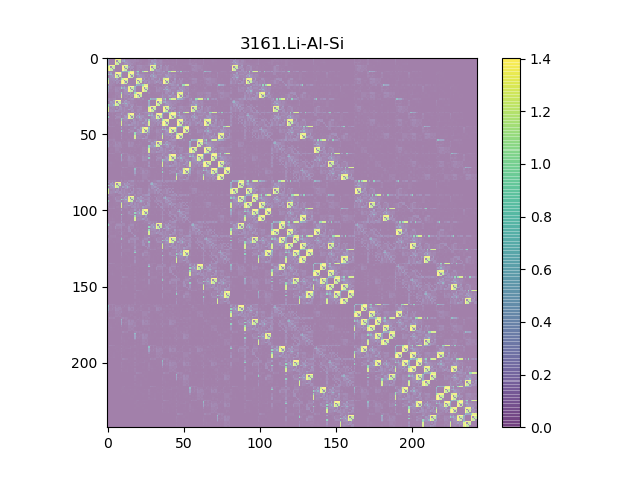
\includegraphics[width=0.85\linewidth]{figures/Crystal_Hamiltonian_GNN_Graph_Neural_Network_for_Hamiltonian_Based_Material_Property_Prediction_p3_1.png}\\
\vspace{1mm}
{\scriptsize 图：Hamiltonian matrix / graph 表示}
\end{columns}
\end{frame}

\begin{frame}[shrink]{MACE：高阶 many-body 等变消息传递}
\small
\begin{itemize}
  \item 正式标题：\textbf{MACE: Higher Order Equivariant Message Passing Neural Networks for Fast and Accurate Force Fields}。
  \item 核心问题：很多等变 GNN 是 2-body，需要较深层数才能逼近高阶相互作用，代价较高。
  \item 关键创新：
  \begin{itemize}
    \item 将 ACE（Atomic Cluster Expansion）与 equivariant MPNN 结合；
    \item 通过高阶消息表达能力，减少对深层网络的依赖；
    \item 在分子力场 benchmark 上达到很强的精度/效率平衡。
  \end{itemize}
  \item 对现有研究基础的启发：
  \begin{itemize}
    \item 如果已跑通 M3GNet，MACE 是继续理解\textbf{等变性 + 高体阶相互作用}的理想下一步；
    \item 后续若做结构弛豫、势函数或 MD，MACE 思想值得借鉴。
  \end{itemize}
  \item 我的理解：MACE 告诉我们：\textbf{高阶物理约束可以替代部分网络深度。}
\end{itemize}
\end{frame}

\section{总结与后续思考}

\begin{frame}[shrink]{本周学习总结：六篇文章对应的三种升级路径}
\small
\begin{itemize}
  \item \textbf{路径一：表示升级 (ComFormer, MGT)}\\
        需要从局部原子图走向\textbf{周期完备表示 + 全局筛选机制}。
  \vspace{1.5mm}
  \item \textbf{路径二：结构升级 (HC-GNN, VGNN)}\\
        图结构本身可以重新设计，包括\textbf{层级超节点}与\textbf{任务驱动虚拟节点}。
  \vspace{1.5mm}
  \item \textbf{路径三：物理约束升级 (Hamiltonian GNN, MACE)}\\
        可从\textbf{更物理的输入对象}和\textbf{更高阶的消息传递}两个方向继续推进。
\end{itemize}

\vspace{1.5mm}
\hrule
\vspace{1.5mm}

\begin{itemize}
  \item \textbf{核心结论}：后续晶体 GNN 改良可以从\textbf{表示、结构、物理}三层同时发力。
\end{itemize}
\end{frame}

\begin{frame}[shrink]{对下一步工作的具体启发}
\begin{enumerate}
  \item 在现有基础中尝试加入 \textbf{global graph 或 transformer block}，验证长程信息的收益；
  \item 设计适合晶体的 \textbf{motif / polyhedron super-node}，探索层级化传播；
  \item 面向声子谱等任务，尝试 \textbf{virtual node + 中间物理对象} 的输出头；
  \item 继续补强 \textbf{物理先验}：如 Hamiltonian-level 表示、many-body 等变消息。
\end{enumerate}

\vspace{1.5mm}
\begin{alertblock}{个人判断}
如果要在当前基础上优先推进，我认为最值得先落地的两条路线是：
\begin{itemize}
  \item \textbf{路线 A}：现有网络 + 全局图 / 长程注意力机制
  \item \textbf{路线 B}：晶体图层级化 + super-node / virtual-node 设计
\end{itemize}
\end{alertblock}
\end{frame}

% ===== 结束页 =====
\begin{frame}
\centering
\Huge 感谢聆听！\\[4mm]
\large 欢迎老师和同学们批评指正
\end{frame}

\end{document}